% THIS IS SIGPROC-SP.TEX - VERSION 3.1
% WORKS WITH V3.2SP OF ACM_PROC_ARTICLE-SP.CLS
% APRIL 2009
%
% It is an example file showing how to use the 'acm_proc_article-sp.cls' V3.2SP
% LaTeX2e document class file for Conference Proceedings submissions.
% ----------------------------------------------------------------------------------------------------------------
% This .tex file (and associated .cls V3.2SP) *DOES NOT* produce:
%       1) The Permission Statement
%       2) The Conference (location) Info information
%       3) The Copyright Line with ACM data
%       4) Page numbering
% ---------------------------------------------------------------------------------------------------------------
% It is an example which *does* use the .bib file (from which the .bbl file
% is produced).
% REMEMBER HOWEVER: After having produced the .bbl file,
% and prior to final submission,
% you need to 'insert'  your .bbl file into your source .tex file so as to provide
% ONE 'self-contained' source file.
%
% Questions regarding SIGS should be sent to
% Adrienne Griscti ---> griscti@acm.org
%
% Questions/suggestions regarding the guidelines, .tex and .cls files, etc. to
% Gerald Murray ---> murray@hq.acm.org
%
% For tracking purposes - this is V3.1SP - APRIL 2009

\documentclass{sig-alternate}
\usepackage{url}
\usepackage{etoolbox}
\usepackage{array}

\usepackage{caption}
\usepackage{wrapfig}

%this removes the copywright message as we dont need it
\patchcmd{\maketitle}{\@copyrightspace}{}{}{}

\begin{document}

\title{Byzantine Fault Tolerance in YARN}

%
% You need the command \numberofauthors to handle the 'placement
% and alignment' of the authors beneath the title.
%

\numberofauthors{4} %  in this sample file, there are a *total*
% of EIGHT authors. SIX appear on the 'first-page' (for formatting
% reasons) and the remaining two appear in the \additionalauthors section.
%
\author{
% You can go ahead and credit any number of authors here,
% e.g. one 'row of three' or two rows (consisting of one row of three
% and a second row of one, two or three).
%
% The command \alignauthor (no curly braces needed) should
% precede each author name, affiliation/snail-mail address and
% e-mail address. Additionally, tag each line of
% affiliation/address with \affaddr, and tag the
% e-mail address with \email.
%
% 1st. author
\alignauthor
Josh Fuerst\\
       \affaddr{Purdue University}\\
       \email{fuerst@purdue.edu}       
% 2nd. author
\alignauthor
Rachna Goyal\\
       \affaddr{Purdue University}\\
       \email{goyal15@purdue.edu}
\and 
% 3rd. author
\alignauthor 
Josh Reese\\
       \affaddr{Purdue University}\\
       \email{reese5@purdue.edu}
% 4th author
\alignauthor 
Derek Schatzlein\\
       \affaddr{Purdue University}\\
       \email{dschatzleinop@gmail.com}
}

\maketitle

\begin{abstract}
Lorem ipsum dolor sit amet, consectetur adipiscing elit. Etiam id mauris adipiscing, pellentesque ligula sit amet, luctus leo. 
Duis congue nisl metus, id pretium nulla auctor vel. Lorem ipsum dolor sit amet, consectetur adipiscing elit. Sed mauris nisl, 
tincidunt nec purus sagittis, condimentum aliquet eros. Pellentesque eu dolor lectus. Nunc gravida, ipsum at pretium mollis, neque 
est porta massa, sed iaculis odio tellus vitae est. Nunc accumsan interdum condimentum. Fusce sit amet neque ut erat commodo molestie id ac est.
\end{abstract}


\section{INTRODUCTION}
Lorem ipsum dolor sit amet, consectetur adipiscing elit. Etiam id mauris adipiscing, pellentesque ligula sit amet, luctus leo. 
Duis congue nisl metus, id pretium nulla auctor vel. Lorem ipsum dolor sit amet, consectetur adipiscing elit. Sed mauris nisl, 
tincidunt nec purus sagittis, condimentum aliquet eros. Pellentesque eu dolor lectus. Nunc gravida, ipsum at pretium mollis, neque 
est porta massa, sed iaculis odio tellus vitae est. Nunc accumsan interdum condimentum. Fusce sit amet neque ut erat commodo molestie id ac est.

Nunc sagittis lacus mattis, lobortis nibh ac, varius justo. Aliquam vestibulum enim et molestie lobortis. Praesent magna nulla, auctor
egestas dictum quis, condimentum quis elit. Pellentesque iaculis bibendum pellentesque. Donec id semper sem. Nulla lacinia in leo fringilla 
laoreet. Integer in purus non nunc dapibus sagittis. Nunc dapibus neque nec ligula pretium, et rhoncus sapien pulvinar. Phasellus a enim rhoncus,
 ultricies tortor ut, vulputate enim. Aliquam odio orci, pharetra tempus ante at, mattis vehicula justo. Donec blandit ligula felis, placerat 
 fermentum nibh mollis sit amet. Nunc sed ultrices leo. Cras ut justo sed lacus accumsan condimentum sit amet in justo. Suspendisse dui diam, 
 venenatis a nisi at, sollicitudin gravida nisi.
 
\section{RELATED WORK}
\label{sec:related}

\begin{table*}
\centering
\begin{tabular}{|>{\bfseries}c|c|c|c|c|c|} \hline
\textbf{Method}    &    \textbf{Park Cost}    &    \textbf{User involvement}    &    \textbf{Accuracy}    &    \textbf{Automated}    &    \textbf{User Visibility}\\ \hline
Landmarks    &    None    &    Passive    &    Low    &    No    &    At Gate\\ \hline
Sensor Systems    &    High    &    Passive    &    High    &    Yes    &    At Gate/Online\\ \hline
Active Mobile Apps    &    None    &    Active    &    High/Low    &    Yes    &    Mobile Device (online)\\ \hline
Our Application    &    None    &    Passive    &    High/Low    &    Yes    &    Mobile Device (online)\\ \hline
\end{tabular}
\caption{Comparison of Queue Tracking Systems}
\label{tab:related_work}
\end{table*}


Lorem ipsum dolor sit amet, consectetur adipiscing elit. Etiam id mauris adipiscing, pellentesque ligula sit amet, luctus leo. 
Duis congue nisl metus, id pretium nulla auctor vel. Lorem ipsum dolor sit amet, consectetur adipiscing elit. Sed mauris nisl, 
tincidunt nec purus sagittis, condimentum aliquet eros. Pellentesque eu dolor lectus. Nunc gravida, ipsum at pretium mollis, neque 
est porta massa, sed iaculis odio tellus vitae est. Nunc accumsan interdum condimentum. Fusce sit amet neque ut erat commodo molestie id ac est.

Nunc sagittis lacus mattis, lobortis nibh ac, varius justo. Aliquam vestibulum enim et molestie lobortis. Praesent magna nulla, auctor
egestas dictum quis, condimentum quis elit. Pellentesque iaculis bibendum pellentesque. Donec id semper sem. Nulla lacinia in leo fringilla 
laoreet. Integer in purus non nunc dapibus sagittis. Nunc dapibus neque nec ligula pretium, et rhoncus sapien pulvinar. Phasellus a enim rhoncus,
 ultricies tortor ut, vulputate enim. Aliquam odio orci, pharetra tempus ante at, mattis vehicula justo. Donec blandit ligula felis, placerat 
 fermentum nibh mollis sit amet. Nunc sed ultrices leo. Cras ut justo sed lacus accumsan condimentum sit amet in justo. Suspendisse dui diam, 
 venenatis a nisi at, sollicitudin gravida nisi.
 
\section {SYSTEM DESIGN}
\label{sec:method}

\begin{figure}
\centering
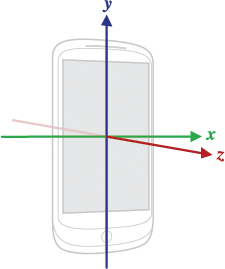
\includegraphics[width=3.5cm]{images/android_axis.png}
\caption{Android Orientation Sensor Axis}
\label{fig:axis}
\end{figure}

Lorem ipsum dolor sit amet, consectetur adipiscing elit. Etiam id mauris adipiscing, pellentesque ligula sit amet, luctus leo. 
Duis congue nisl metus, id pretium nulla auctor vel. Lorem ipsum dolor sit amet, consectetur adipiscing elit. Sed mauris nisl, 
tincidunt nec purus sagittis, condimentum aliquet eros. Pellentesque eu dolor lectus. Nunc gravida, ipsum at pretium mollis, neque 
est porta massa, sed iaculis odio tellus vitae est. Nunc accumsan interdum condimentum. Fusce sit amet neque ut erat commodo molestie id ac est.

Nunc sagittis lacus mattis, lobortis nibh ac, varius justo. Aliquam vestibulum enim et molestie lobortis. Praesent magna nulla, auctor
egestas dictum quis, condimentum quis elit. Pellentesque iaculis bibendum pellentesque. Donec id semper sem. Nulla lacinia in leo fringilla 
laoreet. Integer in purus non nunc dapibus sagittis. Nunc dapibus neque nec ligula pretium, et rhoncus sapien pulvinar. Phasellus a enim rhoncus,
 ultricies tortor ut, vulputate enim. Aliquam odio orci, pharetra tempus ante at, mattis vehicula justo. Donec blandit ligula felis, placerat 
 fermentum nibh mollis sit amet. Nunc sed ultrices leo. Cras ut justo sed lacus accumsan condimentum sit amet in justo. Suspendisse dui diam, 
 venenatis a nisi at, sollicitudin gravida nisi.
 

\section {EVALUATION}
\label{sec:evaluation}
Lorem ipsum dolor sit amet, consectetur adipiscing elit. Etiam id mauris adipiscing, pellentesque ligula sit amet, luctus leo. 
Duis congue nisl metus, id pretium nulla auctor vel. Lorem ipsum dolor sit amet, consectetur adipiscing elit. Sed mauris nisl, 
tincidunt nec purus sagittis, condimentum aliquet eros. Pellentesque eu dolor lectus. Nunc gravida, ipsum at pretium mollis, neque 
est porta massa, sed iaculis odio tellus vitae est. Nunc accumsan interdum condimentum. Fusce sit amet neque ut erat commodo molestie id ac est.

Nunc sagittis lacus mattis, lobortis nibh ac, varius justo. Aliquam vestibulum enim et molestie lobortis. Praesent magna nulla, auctor
egestas dictum quis, condimentum quis elit. Pellentesque iaculis bibendum pellentesque. Donec id semper sem. Nulla lacinia in leo fringilla 
laoreet. Integer in purus non nunc dapibus sagittis. Nunc dapibus neque nec ligula pretium, et rhoncus sapien pulvinar. Phasellus a enim rhoncus,
 ultricies tortor ut, vulputate enim. Aliquam odio orci, pharetra tempus ante at, mattis vehicula justo. Donec blandit ligula felis, placerat 
 fermentum nibh mollis sit amet. Nunc sed ultrices leo. Cras ut justo sed lacus accumsan condimentum sit amet in justo. Suspendisse dui diam, 
 venenatis a nisi at, sollicitudin gravida nisi.
 

\section{LIMITATIONS AND FUTURE WORK}
\label{sec:future}
Lorem ipsum dolor sit amet, consectetur adipiscing elit. Etiam id mauris adipiscing, pellentesque ligula sit amet, luctus leo. 
Duis congue nisl metus, id pretium nulla auctor vel. Lorem ipsum dolor sit amet, consectetur adipiscing elit. Sed mauris nisl, 
tincidunt nec purus sagittis, condimentum aliquet eros. Pellentesque eu dolor lectus. Nunc gravida, ipsum at pretium mollis, neque 
est porta massa, sed iaculis odio tellus vitae est. Nunc accumsan interdum condimentum. Fusce sit amet neque ut erat commodo molestie id ac est.

Nunc sagittis lacus mattis, lobortis nibh ac, varius justo. Aliquam vestibulum enim et molestie lobortis. Praesent magna nulla, auctor
egestas dictum quis, condimentum quis elit. Pellentesque iaculis bibendum pellentesque. Donec id semper sem. Nulla lacinia in leo fringilla 
laoreet. Integer in purus non nunc dapibus sagittis. Nunc dapibus neque nec ligula pretium, et rhoncus sapien pulvinar. Phasellus a enim rhoncus,
 ultricies tortor ut, vulputate enim. Aliquam odio orci, pharetra tempus ante at, mattis vehicula justo. Donec blandit ligula felis, placerat 
 fermentum nibh mollis sit amet. Nunc sed ultrices leo. Cras ut justo sed lacus accumsan condimentum sit amet in justo. Suspendisse dui diam, 
 venenatis a nisi at, sollicitudin gravida nisi.
 
\section{CONCLUSIONS}
\label{sec:conclusions}
Lorem ipsum dolor sit amet, consectetur adipiscing elit. Etiam id mauris adipiscing, pellentesque ligula sit amet, luctus leo. 
Duis congue nisl metus, id pretium nulla auctor vel. Lorem ipsum dolor sit amet, consectetur adipiscing elit. Sed mauris nisl, 
tincidunt nec purus sagittis, condimentum aliquet eros. Pellentesque eu dolor lectus. Nunc gravida, ipsum at pretium mollis, neque 
est porta massa, sed iaculis odio tellus vitae est. Nunc accumsan interdum condimentum. Fusce sit amet neque ut erat commodo molestie id ac est.

Nunc sagittis lacus mattis, lobortis nibh ac, varius justo. Aliquam vestibulum enim et molestie lobortis. Praesent magna nulla, auctor
egestas dictum quis, condimentum quis elit. Pellentesque iaculis bibendum pellentesque. Donec id semper sem. Nulla lacinia in leo fringilla 
laoreet. Integer in purus non nunc dapibus sagittis. Nunc dapibus neque nec ligula pretium, et rhoncus sapien pulvinar. Phasellus a enim rhoncus,
 ultricies tortor ut, vulputate enim. Aliquam odio orci, pharetra tempus ante at, mattis vehicula justo. Donec blandit ligula felis, placerat 
 fermentum nibh mollis sit amet. Nunc sed ultrices leo. Cras ut justo sed lacus accumsan condimentum sit amet in justo. Suspendisse dui diam, 
 venenatis a nisi at, sollicitudin gravida nisi.
 

% The following two commands are all you need in the
% initial runs of your .tex file to
% produce the bibliography for the citations in your paper.
\bibliographystyle{abbrv}
\bibliography{references}  % references.bib is the name of the Bibliography in this case

\balancecolumns
\end{document}